\documentclass[a4paper,12pt]{article}
\usepackage[title]{appendix}
\usepackage{listings,amsmath,amssymb,xcolor,graphicx,url,natbib}
\usepackage{amsfonts}
\usepackage[inner=3cm,outer=3cm,top=3cm,bottom=3cm]{geometry}
\definecolor{lgrey}{HTML}{808080}
\definecolor{dgrey}{HTML}{404040}
\usepackage[framed,numbered,autolinebreaks,useliterate]{mcode}
\usepackage{cases}
\usepackage{color}
\usepackage{bm}



% \inline is a custom macro
\def\inline{\lstinline[basicstyle=\ttfamily]}

% \includecode is a custom macro
% usage is:
% \includecode{title}{filename}
% where 'title' is the displayed title of the file (usually its name)
%   and 'filename' is the full filename, including the path relative to the LaTeX document
% See example below in the appendix
\newcommand{\includecode}[2]{\subsection{\lstinline[basicstyle=\ttfamily\large]{#1}}\lstinputlisting{#2}}



% Document title: uncomment the appropriate title
\title{Linear Stability}
%\title{Coursework 2}
%\title{Coursework 3}
%\title{Project 1: (Project name)} % add the name of the project
%\title{Project 2: (Project name)} % add the name of the project

\author{Hao Ye} % your student number here
%\date{2023.4.20}


\begin{document}
\maketitle
%% Document body starts here

In this file, we present all the theoretical aspects underlying this project, including sections on mathematical modelling and its implementation.

\section{Fluid-solid interaction}
We have reduced the dimensions of the problem from three to two. Generally speaking, we will investigate a two-dimensional problem concerning the deformation and motion of a slender elastic particle in shear flow at a low Reynolds number, focussing on the particle's orientation and trajectory when it reaches equilibrium in the fluid. As this project concerns both fluid and solid mechanics, we will introduce these two components separately and then integrate them to discuss the fluid-solid interaction.
\subsection{Fluid mechanics}
We set the undeformed slender elastic particle clamped at the origin of the laboratory reference frame $\{\mathbf{e'_1}, \mathbf{e'_2}, \mathbf{e'_3}\}$ as
$\mathbf{r}_0^*(\xi^*)=(0,\xi^*)^T$, where $\xi^*\in [0,\mathcal{L}]$. We then assume that its deformed state is given by $\mathbf{R}_0^*(t^*,\xi^*)$. 
Final position of the deformed particle after translation and rotation is determined as follows:
\begin{equation}
	\label{eqn:19}
	\mathbf{R}^*(t^*,\xi^*)=\bm{\mathcal{R}}\,\mathbf{R}_0^*(t^*,\xi^*)+\mathbf{r}_b^*(t^*),
\end{equation}
where $\bm{\mathcal{R}}=\left(\begin{aligned}
	&\cos(\phi(t))\quad -\sin(\phi(t)) \\
	&\sin(\phi(t))\quad \cos(\phi(t))
\end{aligned}\right)$ is the rotation matrix with $\phi(t)$ which measures the particle's inclination as shown in Figure \ref{fig:5}, and $\textbf{r}_b^*(t^*)$ represents the translation of the particle. Note that inclination $\phi(t)$ refers to the actual rotational angle of the object. From Figure \ref{fig:5}, we can easily derive the relationship between orientation and inclination as follows:
\begin{equation}
	\label{eqn:20}
	\theta(t)=\frac{\pi}{2}-\phi(t).
\end{equation}
\begin{figure}[htb]
	\begin{center}
		% specify width as 80% of the width of the text on the page
		% we can also specify a width in centimetres, e.g. [width=8cm]
		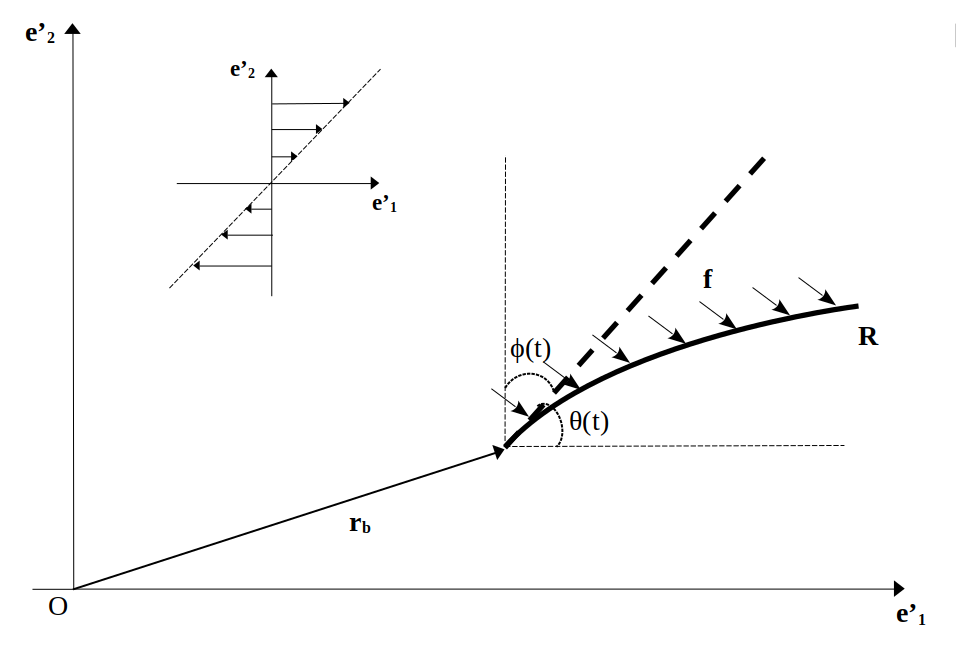
\includegraphics[width=1\textwidth]{plot/fluid_general.png}
		\caption{Schematic of a slender elastic particle in the deformed state in shear flow. The dashed black line represents its undeformed configuration.}
		\label{fig:5}
	\end{center}
	%	\setlength{\abovecaptionskip}{-0.5 cm}
\end{figure}
Since we consider a slender elastic particle immersed in shear flow, the velocity of the background flow is given by
\begin{equation}
	\label{eqn:21}
	\mathbf{U}^{\infty*}(\mathbf{R}^*(t^*,\xi^*))=\dot{\gamma}\left(\mathbf{R}^*(t^*,\xi^*)\cdot\mathbf{e}_y\right)\cdot\mathbf{e}_x,
\end{equation}
where $\mathbf{e}_x=(1,0)^T$ and $\mathbf{e}_y=(0,1)^T$ are both unit vectors. Then, the particle's velocity from kinematics is 
\begin{equation}
	\label{eqn:22}
	\mathbf{U}^*=\frac{\partial\mathbf{R}^*(t^*,\xi^*)}{\partial t^*}.
\end{equation}
Let us define a tangential vector to surface of the particle:
\begin{equation}
	\label{eqn:23}
	\mathbf{e}_t=\frac{1}{|\frac{\partial\mathbf{R}^*(t^*,\xi^*)}{\partial\xi^*}|}\frac{\partial\mathbf{R}^*(t^*,\xi^*)}{\partial\xi^*}.
\end{equation}
From the slender body theory, the traction is obtained as flows:
\begin{equation}
	\label{eqn:24}
	\mathbf{f}^*=c_\perp\left(\mathbf{I}-\frac{1}{2}\mathbf{e}_t\mathbf{e}_t\right)\cdot(\mathbf{U}^{\infty*}-\mathbf{U}^*),
\end{equation}
where $c_\perp=\frac{4\pi\mu}{\ln{\frac{1}{\epsilon}}}$ is the drag coefficient. 

We non-dimensionalise the variables mentioned in this section using the following basic relationships (we set the total length
of the particle as the characteristic length $\mathcal{L}$ and define the time scale as $\frac{1}{\dot{\gamma}}$ , where $\dot{\gamma}$ is the shear rate.) :
\begin{equation}
	\label{eqn:25}
	\xi^*=\mathcal{L}\xi, \quad t^*=\frac{1}{\dot{\gamma}}\,t,
\end{equation}
where the non-dimensional variables are identified without asterisks.
Hence, the relationship between dimensional and non-dimensional variables are given by
\begin{equation}
	\label{eqn:26}
	(\mathbf{r}_0^*, \mathbf{r}_b^*, \mathbf{R}_0^*, \mathbf{R}^*)^T=\mathcal{L}\cdot(\mathbf{r}_0, \mathbf{r}_b, \mathbf{R}_0, \mathbf{R})^T,
\end{equation}
\begin{equation}
	\label{eqn:27}
	\mathbf{U}^{\infty*}=\mathcal{L}\dot{\gamma}\mathbf{U}^{\infty}, \quad \mathbf{U}^*=\mathcal{L}\dot{\gamma}\mathbf{U},
\end{equation}
\begin{equation}
	\label{eqn:28}
	\mathbf{f}^*=c_\perp\,\mathcal{L}\,\dot{\gamma}\,\left(\mathbf{I}-\frac{1}{2}\mathbf{e}_t\mathbf{e}_t\right)\cdot(\mathbf{U}^{\infty}-\mathbf{U})=c_\perp\,\mathcal{L}\,\dot{\gamma}\,\mathbf{f}_{f},
\end{equation}
where 
\begin{equation}
	\label{eqn:101}
	\begin{aligned}
	\mathbf{f}_f=&\left(\mathbf{I}-\frac{1}{2}\mathbf{e}_t\mathbf{e}_t\right)\cdot(\mathbf{U}^{\infty}(t)-\mathbf{U}(t))\\
	=&\left(\mathbf{I}-\frac{1}{2}\mathbf{e}_t\mathbf{e}_t\right)\cdot\Big((\bm{\bm{R}}(t,\xi)\cdot\textbf{e}_y)\cdot\textbf{e}_x-\frac{\partial\textbf{R}(t,\xi)}{\partial t}\Big)
	\end{aligned}
\end{equation}
is the non-dimensional fluid traction. Considering the second term of \eqref{eqn:101},
\begin{equation}
	\label{eqn:120}
	\begin{aligned}
	&(\bm{R}(t,\xi)\cdot\textbf{e}_y)\cdot\textbf{e}_x-\frac{\partial\textbf{R}(t,\xi)}{\partial t}=\\
	&\left(
	\begin{aligned}	
		&-cos(\phi)\,\dot{R}_0^1+sin(\phi)\,\dot{R}_0^2+\Big(sin(\phi)\,R_0^1+cos(\phi)\,R_0^2\Big)\dot{\phi}+sin(\phi)\,R_0^1+cos(\phi)\,R_0^2-\dot{X_0}+Y_0\\
		&-\dot{\phi}\,cos(\phi)\,R_0^1-sin(\phi)\,\dot{R}_0^1+\dot{\phi}\,sin(\phi)\,R_0^2-cos(\phi)\,\dot{R}_0^2-\dot{Y}_0
	\end{aligned}\right),
\end{aligned}
\end{equation}
where $\bm{R}_0(t,\xi)=\left(\begin{aligned}
	&R_0^1(t,\xi) \\
	&R_0^2(t,\xi)
\end{aligned}\right)$ and $\bm{r}_b(t)=\left(\begin{aligned}
	&X_0(t) \\
	&Y_0(t)
\end{aligned}\right)$.




\subsection{Solid mechanics}
We are considering the fluid-solid interaction, so next we will focus on the part related to solid mechanics. This report employs geometrically nonlinear Kirchhoff-Love beam theory with incrementally linear constitutive equations to describe the deformation issues of elastic beams subjected to forces in fluid. We define the deformation of the beam as the dimensionless centreline displacement, $\bm{\omega} = \frac{\bm{\omega}^*}{\mathcal{L}}$. The position of a material point on the beam's centerline is denoted by 
\begin{equation}
	\label{eqn:61}
	\mathbf{r}_0(\xi^1, \xi^2=0)=\mathbf{r}^0_0(\xi^1),\quad \xi^1\in [0,1].
\end{equation}
Then the position of an arbitrary point in the undeformed beam is given by 
\begin{equation}
	\label{eqn:62}
	\mathbf{r}_0(\xi^1, \xi^2)=\mathbf{r}^0_0(\xi^1)+\xi^2\mathbf{n},\quad \xi^2\in [-\frac{h}{2},\frac{h}{2}],
\end{equation}
where $\mathbf{n}=(1,0)^T$ is the normal vector to the undeformed centerline, and $\frac{h}{2}=\frac{h^*}{2\mathcal{L}}$ is the non-dimensional radius of the cross section of the beam. After the deformation, the previous position $\mathbf{r}^0_0(\xi^1)$ in the undeformed reference configuration is transformed to a new position 
\begin{equation}
	\label{eqn:63}
	\mathbf{R}^0_0(\xi^1)=\mathbf{r}^0_0(\xi^1)+\bm{\omega}(\xi^1).
\end{equation}
We decompose the displacement $\bm{\omega}$ into the undeformed basis:
\begin{equation}
	\label{eqn:64}
	\bm{\omega}=\omega^1\mathbf{a}_1+\omega^2\mathbf{a}_2,
\end{equation}
where $\mathbf{a}_1=\frac{\partial \mathbf{r}^0_0}{\partial\xi^1}$ and $\mathbf{a}_3=\mathbf{n}$. The Kirchhoff-Love assumption states that material lines, which were normal to the undeformed centreline, remain normal to the deformed centreline and remain unstretched. Therefore, an arbitrary material point $\mathbf{r}_0$ after deformation is given by 
\begin{equation}
	\label{eqn:65}
	\mathbf{R}_0(\xi^1,\xi^2)=\mathbf{R}^0_0(\xi^1)+\xi^2\mathbf{N},
\end{equation}
where $\mathbf{N}$ is the normal to the deformed configuration.

We then give the non-dimensional equation by scaling the stresses and the applied traction on the beam's effective Young's modulus
\begin{equation}
	\label{eqn:29}
	E_{eff}=\frac{E}{(1-v^2)},
\end{equation}
where $E$ is the Young's modulus and $v$ is the Poisson ratio. Thus, the dimensional and non-dimensional variables are related by 
\begin{equation}
	\label{eqn:30}
	\left(\begin{aligned}
		&\mathbf{f^*} \\
		&\mathbf{\sigma}_0^*
	\end{aligned}\right)
	=E_{eff}\left(\begin{aligned}
		&\textbf{f}_{s} \\
		&\mathbf{\sigma}_0
	\end{aligned}\right),
\end{equation}
where $\textbf{f}_{s}$ is the non-dimensional solid traction and $\sigma^*_0$ indicates the prestress of the elastic beam.
The non-dimensional form of the principle of virtual displacements that governs the beams deformation is then given by
\begin{equation}
	\label{eqn:31}
	\int^1_0 \left[(\sigma_0+\gamma)\delta\gamma+\frac{1}{12}h^2\kappa\delta\kappa-\left(\frac{1}{h}\sqrt{\frac{A}{a}}\,\textbf{f}_{s}-\Lambda^2\frac{\partial^2\textbf{R}_0}{\partial t^2}
	\right)\cdot \delta \textbf{R}_0
	\right]\,\sqrt{a}\,d\xi=0,
\end{equation}
where 
\begin{equation}
	\label{eqn:32} a=\frac{\partial\textbf{r}_0}{\partial\xi}\cdot\frac{\partial\textbf{r}_0}{\partial\xi}, A=\frac{\partial\textbf{R}_0}{\partial\xi}\cdot\frac{\partial\textbf{R}_0}{\partial\xi}
\end{equation}
denote the squares of the lengths of infinitesimal material line elements in the undeformed and deformed configurations, respectively.
Also, considering undeformed and deformed ones, we have 
\begin{equation}
	\label{eqn:33}
	ds=\sqrt{a}\,d\xi,\,dS=\sqrt{A}\,d\xi.
\end{equation}
$A$ and $a$ could be understood as the "$1\times1$ metric tensors" of the beam's centerline, representing the deformed and undeformed configurations, respectively. 
The ratio $\sqrt{\frac{A}{a}}$ signifies the "extension ratio" or "stretch" of the beam's centerline. We define the curvature of the beam's centerline prior to and following deformation as represented by 
\begin{equation}
	\label{eqn:34}
	b=\textbf{n}\cdot\frac{d^2\textbf{r}_0}{d\xi^2},\,B=\textbf{N}\cdot\frac{\partial^2\textbf{R}_0}{\partial\xi^2}.
\end{equation}
The "$1\times1$" strain and bending "tensors" $\gamma$ and $\kappa$ are obtained by
\begin{equation}
	\label{eqn:35}
	\gamma=\frac{1}{2}(A-a),\,\kappa=-(B-b).
\end{equation}
In $\eqref{eqn:31}$,
\begin{equation}
	\label{eqn:36}
	\Lambda=\mathcal{L}\,\dot{\gamma}\sqrt{\frac{\rho}{E_{eff}}}
\end{equation}
represents the ratio of the natural timescale of the beam's in-plane extensional oscillations. 
$\Lambda^2$ can be treated as the non-dimensional wall density, implying that $\Lambda=0$ signifies the absence of wall inertia.

Since the elastic beam is initially clamped at the origin, the boundary conditions are
\begin{equation}
	\label{eqn:58}
	\begin{aligned}
	&\mathbf{R}_0(\xi=0)\cdot\mathbf{e}_x=0,\\
	&\mathbf{R}_0(\xi=0)\cdot\mathbf{e}_y=0,\\
	&\frac{d\left(\mathbf{R}_0(\xi=0)\cdot\mathbf{e}_x\right)}{d\xi}=0.
	\end{aligned}
\end{equation}

\subsection{Fluid–solid coupling}
The no-slip boundary condition requires that the velocity of the fluid on the surface of the beam $\mathbf{u}$ matches the velocity of the beam at that location. Hence, the boundary condition is 
\begin{equation}
	\label{eqn:100}
	\mathbf{u}=\frac{\partial \mathbf{R}(t,\xi)}{\partial t}.
\end{equation}

Recall that in $\eqref{eqn:28}$, we use slender body theory to evaluate the traction exerted by the fluid on the beam as
\begin{equation}
	\label{eqn:102}
	\mathbf{f}^*=c_\perp\,\mathcal{L}\,\dot{\gamma}\,\mathbf{f}_{f}.
\end{equation}
From \eqref{eqn:30}, the applied traction on beam is 
\begin{equation}
	\label{eqn:103}
	\mathbf{f}^*=E_{eff}\,\mathbf{f}_{s}.
\end{equation}
Hence, the fluid applies traction to the beam, and the loading term in the solid equation \eqref{eqn:31} are expressed by
\begin{equation}
	\label{eqn:37}
	\textbf{f}_{s}=\frac{c_\perp\,\mathcal{L}\,\dot{\gamma}}{E_{eff}}\,\textbf{f}_{f}.
\end{equation}
Then, we define the coefficient in \eqref{eqn:37} as $\mathcal{I}$, which represents the coefficient of fluid-solid interaction and is expressed as:
\begin{equation}
	\label{eqn:38}
	\mathcal{I}=\frac{c_\perp\,\mathcal{L}\,\dot{\gamma}}{E_{eff}}.
\end{equation}
This coefficient, also known as the FSI coefficient, quantifies the degree or strength of the interaction between the fluid and the solid within the system.




\section{Equilibrium equations}
Initially, the elastic beam is clamped at the origin, denoted by $\textbf{r}_0(\xi)=(0,\xi)^T,\,\xi\in [0,1]$. Next, a traction $\mathbf{f}_s=\mathcal{I}\,\textbf{f}_0$  is applied to it, causing deformation denoted as $\textbf{R}_0(t,\xi)$. Substituting 
$\textbf{r}_0(\xi), \textbf{f}_s$ and $\textbf{R}_0(t,\xi)$ into the beam's governing equation $\eqref{eqn:31}$, we obtain the following equation:
\begin{equation}
	\label{eqn:48}
	\bm{\mathcal{S}}\Big(\textbf{R}_0(t,\xi);\textbf{f}_0,\textbf{r}_0(\xi)\Big)=0,
\end{equation}
where $\textbf{R}_0(t,\xi)$ is the unknown and $\bm{\mathcal{S}}(\cdot)$ indicates the left hand side of $\eqref{eqn:31}$.
Subsequently, according to $\eqref{eqn:19}$, a translation and rotation are applied to 
$\textbf{R}_0(t,\xi)$, yielding $\textbf{R}(t,\xi)$ as:
\begin{equation}
	\label{eqn:49}
	\textbf{R}(t,\xi)=\bm{\mathcal{R}}(t)\,\textbf{R}_0(t,\xi)+\textbf{r}_b(t).
\end{equation}
 We compute the fluid traction $\textbf{f}_f$ acting on the beam $\textbf{R}(t,\xi)$ based on $\eqref{eqn:120}$. Then, we rotate this fluid traction $\textbf{f}_f$ back by angle $\phi(t)$ while keeping its magnitude unchanged, obtaining traction $\textbf{f}_0$. Hence, the relationship between $\textbf{f}_0$ and $\textbf{f}_f$ is 
\begin{equation}
	\label{eqn:50}
	\textbf{f}_0=\bm{\mathcal{R}}^{-1}\,\textbf{f}_f,
\end{equation}
where $\bm{\mathcal{R}}^{-1}$ is the inverse of the rotation matrix. Then, the solid traction, which serves as the loading term in the beam equation, is represented as 
\begin{equation}
	\label{eqn:67}
	\textbf{f}_s=\mathcal{I}\,\textbf{f}_0=\mathcal{I}\,\left(\bm{\mathcal{R}}^{-1}\,\textbf{f}_f\right).
\end{equation}
Then $\eqref{eqn:48}$ can be updated by
\begin{equation}
	\label{eqn:51}
	\bm{\mathcal{S}}\Big(\textbf{R}_0(t,\xi), X_0(t), Y_0(t),\phi(t);\textbf{r}_0(\xi)\Big)=0,
\end{equation}
where $\textbf{r}_0(\xi)=(0,\xi)^T,\,\xi\in [0,1]$ is not the unknown in this equation.

The net drag and net torque acting on the beam $\textbf{R}(t,\xi)$ in non-dimensional form are 
\begin{equation}
	\label{eqn:52}
	\textbf{F}=\int^1_0 \textbf{f}\, \left|\frac{\partial\textbf{R}}{\partial\xi}\right|\,d\xi, 
\end{equation}
\begin{equation}
	\label{eqn:53}
	\mathbf{T}\cdot\textbf{e}_z=\left\{\int^1_0 \left[(\textbf{R}-\textbf{R}_{centre})\times \textbf{f}\,\right]\,\left|\frac{\partial\textbf{R}}{\partial\xi}\right|\,d\xi\right\}\cdot\textbf{e}_z,
\end{equation}
where 
\begin{equation}
	\label{eqn:54}
	\textbf{R}_{centre}=\int^1_0 \textbf{R}\,|\frac{\partial\textbf{R}}{\partial\xi}|\,d\xi
\end{equation}
represents the position of centre of mass. The net drag and net torque experienced by the beam are both zero. Hence, we have 
\begin{equation}
	\label{eqn:55}
	\textbf{F}\,\Big(\textbf{R}_0(t,\xi), X_0(t), Y_0(t), \phi(t)\Big)=\textbf{0},
\end{equation}
\begin{equation}
	\label{eqn:56}
	\{\mathbf{T}\cdot\textbf{e}_z\}\,\Big(\textbf{R}_0(t,\xi), X_0(t), Y_0(t), \phi(t)\Big)=0.
\end{equation} 
Combining $\eqref{eqn:51}, \eqref{eqn:55}$ and $\eqref{eqn:56}$, we collect the following equations for unkonwns:
\begin{equation}
	\label{eqn:57}
	\left\{\begin{aligned}
		&\bm{\mathcal{S}}\Big(\textbf{R}_0(t,\xi), X_0(t), Y_0(t),\phi(t);\textbf{r}_0(\xi)\Big)=0\\
		&\textbf{F}\,\Big(\textbf{R}_0(t,\xi), X_0(t), Y_0(t),\phi(t)\Big)=\textbf{0}\\
		&\{\mathbf{T}\cdot\textbf{e}_z\}\,\Big(\textbf{R}_0(\xi), X_0(t), Y_0(t),\phi(t)\Big)=0
	\end{aligned}\right.\Longrightarrow \Big(\textbf{R}_0(t,\xi), X_0(t), Y_0(t),\phi(t)\Big).
\end{equation}

\section{Linear stability}
To facilitate the analysis of the equations, we recall the expressions of solid traction \eqref{eqn:67} and beam equation  \eqref{eqn:48} here:
\begin{equation}
	\label{eqn:104}
		\textbf{f}_s=\mathcal{I}\,\left(\bm{\mathcal{R}}^{-1}\,\textbf{f}_f\right),
\end{equation}
where fluid traction from the slender body theory is 
\begin{equation}
	\label{eqn:105}
	\begin{aligned}
		\textbf{f}_f=&\left(\mathbf{I}-\frac{1}{2}\mathbf{e}_t\mathbf{e}_t\right)\cdot(\mathbf{U}^{\infty}(t)-\mathbf{U}(t))\\
		=&\left(\mathbf{I}-\frac{1}{2}\mathbf{e}_t\mathbf{e}_t\right)\cdot\Big((\bm{\bm{R}}(t,\xi)\cdot\textbf{e}_y)\cdot\textbf{e}_x-\frac{\partial\textbf{R}(t,\xi)}{\partial t}\Big),
	\end{aligned}
\end{equation}
$\mathcal{I}$ is the FSI parameter and  $\bm{\mathcal{R}}^{-1}=\left(\begin{aligned}
	&\cos(\phi(t))\quad \sin(\phi(t)) \\
	&-\sin(\phi(t))\quad \cos(\phi(t))
\end{aligned}\right)$ is the inverse of rotation matrix with $\phi(t)$ which measures the particle's inclination as shown in Figure \ref{fig:5}. We also remind that 
\begin{equation}
	\label{eqn:49}
	\textbf{R}(t,\xi)=\bm{\mathcal{R}}\,\textbf{R}_0(t,\xi)+\textbf{r}_b(t),
\end{equation}
where $\bm{\mathcal{R}}=\left(\begin{aligned}
	&\cos(\phi(t))\quad -\sin(\phi(t)) \\
	&\sin(\phi(t))\quad \cos(\phi(t))
\end{aligned}\right)$ is the rotation matrix and $\bm{r}_b(t)=\left(\begin{aligned}
&X_0(t) \\
&Y_0(t)
\end{aligned}\right)$ is the base vector indicating translation.
Then, the implicit expression of beam equation is 
\begin{equation}
	\label{eqn:106}
	\bm{\mathcal{S}}\Big(\textbf{R}_0(t,\xi),\textbf{f}_s;\textbf{r}_0(\xi)\Big)=0.
\end{equation}
From these expressions above, we find that the three motion unknowns, $X_0(t), Y_0(t)$ and $\phi(t)$, along with their time derivatives,  $\frac{dX_0}{dt}, \frac{dY_0}{dt}$ and $\frac{d\phi}{dt}$, arise solely from the solid traction in the beam equation, namely 	
\begin{equation}
	\label{eqn:107}
\bm{\mathcal{S}}\Big\{\textbf{R}_0(t,\xi),\textbf{f}_s\Big(X_0(t), Y_0(t),\phi(t),\frac{dX_0}{dt}, \frac{dY_0}{dt},\frac{d\phi}{dt}\Big);\textbf{r}_0(\xi)\Big\}=0.
\end{equation}

Since we use the finite element method to solve the equations, the position $\textbf{R}_0(t,\xi)$ has been discretised as the Galerkin solution. In the element level, we have
\begin{equation}
	\label{eqn:108}
R_{0\,(e)}^i=\sum R_{ijk}(t)\, \psi_{jk}(s),
\end{equation}
where $R_{ij1}$ represents the $i$-th coordinate of the local node $j$ and $R_{ij2}$ represents the derivative of $i$-th coordinate with respect to local variable $s$, evaluated at the node local $j$.

We set the governing equations \eqref{eqn:57} as $\bm{E}$ and the unknowns as $\bm{X}=\{R_{ijk}(t),X_0(t), Y_0(t),\phi(t)\}$. Then, applying Taylor's expansion at the base state, we obtain:
\begin{equation}
	\label{eqn:109}
\bm{E}(\bm{X})=\bm{E}(\bar{\bm{X}}+\epsilon \hat{\bm{X}})=\bm{E}(\bar{\bm{X}})+\epsilon \Big(\frac{\partial \bm{E}}{\partial \bm{X}}\Big|_{\bm{X}=\bar{\bm{X}}}\hat{\bm{X}}+\frac{\partial \bm{E}}{\partial \dot{\bm{X}}}\Big|_{\bm{X}=\bar{\bm{X}}}\dot{\hat{\bm{X}}}\Big)+o(\epsilon),
\end{equation}
where $\bar{\bm{X}}$ is the base state, $\hat{\bm{X}}$ is the perturbation and $\epsilon$ is the amplitude of the (initial) perturbation. Since $\bm{E}(\bar{\bm{X}})=\bm{0}$, we have 
\begin{equation}
	\label{eqn:110}
	\frac{\partial \bm{E}}{\partial \bm{X}}\Big|_{\bm{X}=\bar{\bm{X}}}\hat{\bm{X}}+\frac{\partial \bm{E}}{\partial \dot{\bm{X}}}\Big|_{\bm{X}=\bar{\bm{X}}}\dot{\hat{\bm{X}}}=\bm{0}.
\end{equation}
We define the Jacobian matrix as $\bm{\mathcal{J}}=\frac{\partial \bm{E}}{\partial \bm{X}}\Big|_{\bm{X}=\bar{\bm{X}}}$ and the mass matrix as $\bm{\mathcal{M}}=\frac{\partial \bm{E}}{\partial \dot{\bm{X}}}\Big|_{\bm{X}=\bar{\bm{X}}}$. Then, the above equation becomes 
\begin{equation}
	\label{eqn:111}
\bm{\mathcal{J}}\hat{\bm{X}}+\bm{\mathcal{M}}\dot{\hat{\bm{X}}}=\bm{0}.
\end{equation}
The specific expressions of the base state in our case are 
\begin{equation}
	\label{eqn:112}
	\bar{\bm{X}}=\left\{\begin{aligned}
		&\bar{X_0}=\frac{1}{2}Vt^2+U_0t+X_{00} \\
		&\bar{Y_0}=Vt+Y_{00} \\
		&\bar{\phi}=\phi_{eq} \\
		&\overline{R_{ijk}}=R_{ijk}^{eq}.
	\end{aligned}\right.	
\end{equation}
This is different from the classic theory, as our base state here is also a function of time, namely $\frac{d\bar{\bm{X}}}{dt}\neq\bm{0}$. In our project, when the particle reaches equilibrium, only its orientation (inclination) attains a steady state, meaning  $\frac{d\theta}{dt}=0$, while the other two motion variables, $X_0(t), Y_0(t)$, remain time-dependent. However, in this so-called "steady" state, the particle undergoes a certain type motion with a parabolic trajectory. Thus, we may regard it as quasi-steady, since any perturbation to the system would disrupt the particle's motion pattern, yet after some time, the system would return to its original motion type. 

We use \texttt{oomph-lib} to implement this procedure. First, we consider the Jacobian matrix. In \texttt{oomph-lib}, the existing function
\begin{lstlisting}
void fill_in_contribution_to_jacobian(Vector<double> &residuals, DenseMatrix<double> &jacobian)
\end{lstlisting}
can be called directly to evaluate the Jacobian matrix at the base state. However, this function automatically sets $\frac{d\bm{X}}{dt}\Big|_{\bm{X}=\bar{\bm{X}}}=\bm{0}$ when solving the eigenproblem, which conflicts with our case. As illustrated above, there are actually two exceptions to this:
\begin{equation}
	\label{eqn:113}
	\left\{\begin{aligned}
		&\bar{X_0}=\frac{1}{2}Vt^2+U_0t+X_{00} \\
		&\bar{Y_0}=Vt+Y_{00} 
	\end{aligned}\right. \Longrightarrow 
\left\{\begin{aligned}
	&\frac{dX_0}{dt}\Big|_{X_0=\bar{X_0}}=Vt+U_0 \\
	&\frac{dY_0}{dt}\Big|_{Y_0=\bar{Y_0}}=V.
\end{aligned}\right.
\end{equation}
From \eqref{eqn:107} we know that these two exceptional terms $\frac{dX_0}{dt},\frac{dY_0}{dt}$ only come from the fluid traction $\bm{f}_f$ in \eqref{eqn:105}. Therefore, we modify the expression for the fluid traction $\bm{f}_f$ to manually impose
\begin{equation}
	\label{eqn:114}
	\left\{\begin{aligned}
		&\frac{dX_0}{dt}\Big|_{X_0=\bar{X_0}}=U_0 \\
		&\frac{dY_0}{dt}\Big|_{Y_0=\bar{Y_0}}=V.
	\end{aligned}\right.
\end{equation}
Note that it is a bit of different from \eqref{eqn:113} because it is evaluated at $t=0$. Since this corresponds to the steady state, we can assign any value for time $t$ without affecting the results. Generally speaking, computing the Jacobian matrix involves the following steps: first, we compute the steady-state solutions, which include the three motion variables and the configuration's position variables. Since the Jacobian matrix (also the mass matrix) must be evaluated at the base state, we copy the steady configuration (position values) as the initial configuration for the unsteady problem (eigenproblem). Note that in the implementation, the three motion variables are different between the steady and unsteady problems. In steady problem, we have $V, U_0, \phi_{eq}$; in unsteady problem, they should be $X_0(t), Y_0(t), \phi(t)$. Hence, we actually only need to copy the steady value of $\phi$ as the initial guess to the unsteady problem, and it is not necessary to apply this process to the other two variables (Here, since steady inclination will be used to compute the mass matrix, we still include this step. For $X_0, Y_0$, their values do not appear in the mass matrix expressions. Moreover, since the Jacobian matrix is computed numerically, the initial values of these two unknowns are insignificant).

Now, let us consider the mass matrix, for which we derive the expressions of its entries in Maple. This means that we should fully understand the structure of the mass matrix. 
Before discussing this, we must determine the size of the mass matrix. For each arm, if there are $N$ global nodes, the number of degrees of freedom would be $4N-3$, as each node has four positional variables, and at the one end (hinge point) three degrees of freedom are pinned according to the boundary conditions \eqref{eqn:58}. Therefore, for two arms (assuming both have the same number of nodes), there are $8N-6$ degrees of freedom. By adding additional three motion unknowns $X_0(t),Y_0(t),\phi(t)$, the system has a total of $8N-3$ degrees of freedom. Hence, the size of the mass matrix (also for the Jacobian matrix) should be $8N-3$ by $8N-3$. Meanwhile, the residues $\bm{E}$ becomes
\begin{equation}
	\label{eqn:116}
	\bm{E}=\{\mathcal{S}_1,\mathcal{S}_2,...,\mathcal{S}_{8N-6},F_1,F_2,T\}_{8N-3}.
\end{equation}

The mass matrix comprises six blocks, with the general structure given by
\begin{equation}
\begin{pmatrix}
	\label{eqn:115}
	\begin{pmatrix}
		\frac{\partial F_1}{\partial\dot{X_0}} & \frac{\partial F_1}{\partial\dot{Y_0}} & \frac{\partial F_1}{\partial\dot{\phi}}\\
		\frac{\partial F_2}{\partial\dot{X_0}} & \frac{\partial F_2}{\partial\dot{Y_0}} & \frac{\partial F_2}{\partial\dot{\phi}}\\
		\frac{\partial T}{\partial\dot{X_0}} & \frac{\partial T}{\partial\dot{Y_0}} & \frac{\partial T}{\partial\dot{\phi}}
	\end{pmatrix}_{3\times 3} & \begin{pmatrix}
	\frac{\partial F_1}{\partial\dot{R_{ijk}^{e,[0]}}} & ...\\
	\frac{\partial F_2}{\partial\dot{R_{ijk}^{e,[0]}}} & ...\\
	\frac{\partial T}{\partial\dot{R_{ijk}^{e,[0]}}} & ...
\end{pmatrix}_{3\times (4N-3)} & \begin{pmatrix}
\frac{\partial F_1}{\partial\dot{R_{ijk}^{e,[1]}}} & ...\\
\frac{\partial F_2}{\partial\dot{R_{ijk}^{e,[1]}}} & ...\\
\frac{\partial T}{\partial\dot{R_{ijk}^{e,[1]}}} & ...
\end{pmatrix}_{3\times (4N-3)}\\
	\begin{pmatrix}
		\frac{\partial\mathcal{S}_1}{\partial\dot{X_0}} & \frac{\partial\mathcal{S}_1}{\partial\dot{Y_0}} & \frac{\partial\mathcal{S}_1}{\partial\dot{\phi}}\\
		\vdots & \vdots & \vdots\\
	\frac{\partial\mathcal{S}_{8N-6}}{\partial\dot{X_0}} & \frac{\partial\mathcal{S}_{8N-6}}{\partial\dot{Y_0}} & \frac{\partial\mathcal{S}_{8N-6}}{\partial\dot{\phi}}
	\end{pmatrix}_{(8N-6)\times 3} & \begin{pmatrix}
	\frac{\partial\mathcal{S}_1}{\partial\dot{R_{ijk}^{e,[0]}}} & ...\\
	\vdots & ...\\
	\frac{\partial\mathcal{S}_{8N-6}}{\partial\dot{R_{ijk}^{e,[0]}}} & ...
\end{pmatrix}_{(8N-6)\times (4N-3)} & \begin{pmatrix}
\frac{\partial\mathcal{S}_1}{\partial\dot{R_{ijk}^{e,[1]}}} & ...\\
\vdots & ...\\
\frac{\partial\mathcal{S}_{8N-6}}{\partial\dot{R_{ijk}^{e,[1]}}} & ...
\end{pmatrix}_{(8N-6)\times (4N-3)}
\end{pmatrix},
\end{equation}
where $R_{ijk}^{e,[0]}$ indicates the positional unknowns in the $e$-th element of the first arm of the particle, similarly for $R_{ijk}^{e,[1]}$.
We denote these blocks as 
\begin{equation}
	\label{eqn:117}
\bm{\mathcal{M}}=\begin{pmatrix}
	B_1 & B_2 & B_3\\
	B_4 & B_5 & B_6
\end{pmatrix}.
\end{equation}
In our code, we define two element classes:
\begin{lstlisting}
	UnsteadyHaoHermiteBeamElement()
\end{lstlisting}
This class contains the positional unknowns and introduces three motion unknowns, $X_0(t), Y(t), \phi(t)$, as external data. We assign the expressions for the entries of block $B_4$ by looping over the external data, while the expressions for blocks $B_5$ and $B_6$ are assigned by looping over the positional data.
\begin{lstlisting}
	UnsteadyRigidBodyElement()
\end{lstlisting}
This class contains only the three motion unknowns as internal data, with the positional unknowns treated as external data. The expressions for the entries of block $B_1$ are assigned by looping over the three internal data, while those for blocks $B_2$ and $B_3$ are assigned by looping over the external (positional) data. However, considering positional data $R_{ijk}^{e,[m]}$, there are several labels needed to be looped, and we cannot call the member function of \textit{HermiteBeamElement()}
\begin{lstlisting}
int oomph::SolidFiniteElement::position_local_eqn(const unsigned &n, const unsigned &k, const unsigned &j) 	
\end{lstlisting}
to determine the local equation number (because now these positional values are the external data in this class). A good way to do it is to loop over the external data, and thus we need to evaluate the mapping between the external data label and those positional data labels.
Now let us consider the external data (positional data) in class \textit{UnsteadyRigidBodyElement()}. Since each node has four positional degrees of freedom, each \textit{external\_data\_pt} contains four \textit{Data} values, ordered as follows:
\begin{equation}
	\label{eqn:118}
	\left\{\begin{aligned}
		&\textit{external\_data\_pt(l)->value(0)} \Longrightarrow \bm{R}\cdot \bm{e}_x\\
		&\textit{external\_data\_pt(l)->value(1)} \Longrightarrow \frac{\partial\bm{R}}{\partial s}\cdot \bm{e}_x\\
		&\textit{external\_data\_pt(l)->value(2)} \Longrightarrow \bm{R}\cdot \bm{e}_y\\
		&\textit{external\_data\_pt(l)->value(3)} \Longrightarrow \frac{\partial\bm{R}}{\partial s}\cdot \bm{e}_y\\
	\end{aligned}\right.,
\end{equation}
where $l$ is the label of the external data.
Several labels need to be looped over: 
arm $m$ (particle has two arms, $m=0,1$), element $e$, position direction $i$ ($i=0,1$), position type $k$ ($k=0,1$), and local node $j$ ($j=0,1$). Additionally, we define $n_1$ and $n_2$ as the number of global nodes in the first ($m=0$) and second ($m=1$) arms, respectively, and $v$ as the $v$-th value of the external data. Thus, our goal now is to write up a function 
\begin{lstlisting}
void external_data_index_and_value_index(const unsigned& m,
const unsigned& e,
const unsigned& j,
const unsigned& i,
const unsigned& k,
unsigned& l,
unsigned& v)	
\end{lstlisting}
so that we can get the corresponding $l,v$ in terms of $m,e,n,i,k$.
The mapping is then established as follows:
\begin{table}[h]
	\centering
	\caption{Mapping.}  
	\label{tab:1}
	\begin{tabular}{ |c|c| } 
		\hline
		$m$ & ...  \\ 
		\hline
		$e$ & ...  \\ 
		\hline
		$j$ & ...  \\ 
		\hline
		$l$ & ... \\
		\hline
	\end{tabular}
\end{table}
where $l\in [0,n_1+n_2)$ and external data label $l$ is determined by arm $m$, element $e$, and local node $j$. Then, the label of values $v$ is only determined by position direction $i$ and position type $k$ according to \eqref{eqn:118}:
\begin{equation}
	\label{eqn:119}
	\text{value}\rightarrow v=\left\{\begin{aligned}
		&0,\quad i=k=0\\
		&1,\quad i=0, k=1\\
		&2,\quad i=1, k=0\\
		&3,\quad i=1, k=1
	\end{aligned}\right.,
\end{equation}
where $v\in [0,3]$. By the way, all labels we mentioned here are non-negative integers. Here, we give an example to illustrate these relationships.
If we set there are 3 elements at each arm, it means there are 4 global nodes at each arm. Then, we offer a plot Figure \ref{fig:6} to explain this example, especially the label of the external data $l$.
\begin{figure}[htb]
	\begin{center}
		% specify width as 80% of the width of the text on the page
		% we can also specify a width in centimetres, e.g. [width=8cm]
		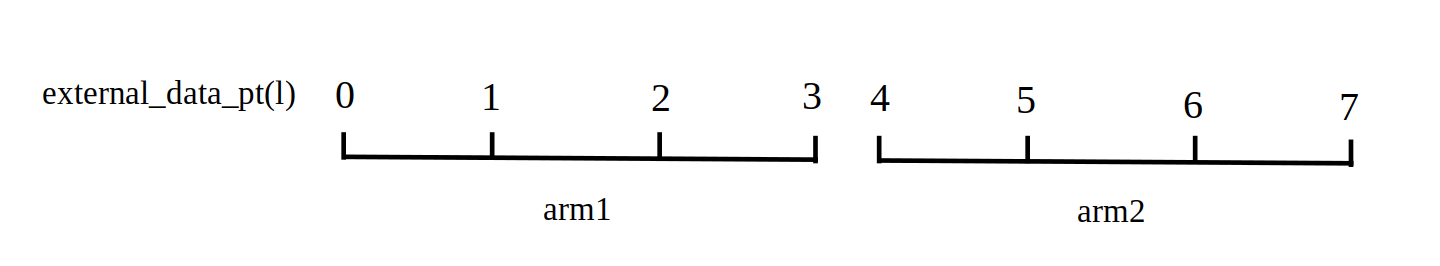
\includegraphics[width=1\textwidth]{plot/example.png}
		\caption{Example of 3 elements for each arm of the particle (numbers in the plot are external data label $l$).}
		\label{fig:6}
	\end{center}
	%	\setlength{\abovecaptionskip}{-0.5 cm}
\end{figure}
In this case, the number of the global nodes in the first and second arms are $n_1=n_2=4$. Thus, according to the relationships Table \ref{tab:1}, we can obtain the Table \ref{tab:2} to show the mapping for this example.
\begin{table}[h]
	\centering
	\caption{The mapping for the example.}  
	\label{tab:2}
	\begin{tabular}{ |c|c|c|c|c|c|c|c|c|c|c|c|c| } 
		\hline
		$m$ & 0 & 0 &0 &0 &0 &0 & 1 & 1 &1 &1 &1 &1 \\ 
		\hline
		$e$ & 0 & 0 &1 &1 &2 &2 & 0 & 0 &1 &1 &2 &2 \\ 
		\hline
		$j$ & 0 & 1 &0 &1 &0 &1 & 0 & 1 &0 &1 &0 &1 \\ 
		\hline
		$l$ & 0 & 1 &1 &2 &2 &3 & 4 & 5 &5 &6 &6 &7 \\ 
		\hline
	\end{tabular}
\end{table}
In addition, $i,k$ are still as \eqref{eqn:119}. We can easily test these above relationships with Figure \ref{fig:6}. Note that element $e$ and local node $j$ should be regarded together. For instance, if $l=2$, the corresponding global node belongs to both element 1 and element 2. When this node is within element 1, its local node is $j=1$, whereas in element 2, its local node is $j=0$. Consequently, in this case, we must iterate over both element 1 and element 2, leading to the superposition of results. By the way, considering the function \textit{add\_external\_data()} which is to add the position variables as the external data to \textit{UnsteadyRigidBodyElement()}, an error may be reported if a node has already been added, but it can still return the index of the external data $l$ and skip this node.

You may find our previous explanation somewhat counterintuitive, given that \textit{UnsteadyRigidBodyElement()} is an element class. However, when assigning expressions to the entries, we actually iterate over all arms and elements. This is because \textit{UnsteadyRigidBodyElement()} only has three internal data. As a result, when computing the three residuals (drag-free and torque-free), we must adopt a global perspective—considering the entire particle. Thus, blocks $B_1,B_2,B_3$ will be a little tricky to assemble since they are conducted in \textit{UnsteadyRigidBodyElement()}. For instance, in the case of $B_1$​, when evaluating $\frac{\partial F_1}{\partial\dot{X_0}}$, we have 
\begin{equation}
	\label{eqn:127}
\frac{\partial F_1}{\partial\dot{X_0}}=\frac{\partial (F_1^{[0]}+F_1^{[1]})}{\partial\dot{X_0}}=\frac{\partial F_1^{[0]}}{\partial\dot{X_0}}+\frac{\partial F_1^{[1]}}{\partial\dot{X_0}}.
\end{equation}
This is the machinery we use, so actually we first compute $\frac{\partial F_1}{\partial\dot{X_0}}$ for a single arm, namely $\frac{\partial F_1^{[m]}}{\partial\dot{X_0}}$. We then iterate over both arms, summing the contributions to obtain the final result. The same procedure is applied to the other entries in block $B_1$​. Then, if we conduct this process to evaluate entries in blocks $B_2,B_3$, we will have, for example:
\begin{equation}
	\label{eqn:128}
	\frac{\partial F_1}{\partial\dot{R_{ijk}^{e,[0]}}}\neq\frac{\partial F_1^{[0]}}{\partial\dot{R_{ijk}^{e,[0]}}}+\frac{\partial F_1^{[1]}}{\partial\dot{R_{ijk}^{e,[1]}}},
\end{equation}
which is not correct because, in block $B_2$, all the entries should be respect to the first arm's terms. However, we can also have 
\begin{equation}
	\label{eqn:129}
	\frac{\partial F_1}{\partial\dot{R_{ijk}^{e,[0]}}}=\frac{\partial( F_1^{[0]}+F_1^{[1]})}{\partial\dot{R_{ijk}^{e,[0]}}}=\frac{\partial F_1^{[0]}}{\partial\dot{R_{ijk}^{e,[0]}}}+\frac{\partial F_1^{[1]}}{\partial\dot{R_{ijk}^{e,[0]}}}=\frac{\partial F_1^{[0]}}{\partial\dot{R_{ijk}^{e,[0]}}},
\end{equation}
where $\frac{\partial F_1^{[1]}}{\partial\dot{R_{ijk}^{e,[0]}}}=0$. This implies that when computing the entries in block $B_2$​, we only evaluate $\frac{\partial F_1}{\partial\dot{R_{ijk}^{e}}}$​​ for a single arm rather than iterating over both arms. A similar reasoning applies to the corresponding entries in block $B_3$. However, $\frac{\partial F_1^{[0]}}{\partial\dot{R_{ijk}^{e,[0]}}}$ is still very special compared with the terms in $B_5$ (eg. $\frac{\partial\mathcal{S}_1}{\partial\dot{R_{ijk}^{e,[0]}}}$). Considering $\frac{\partial\mathcal{S}_1}{\partial\dot{R_{ijk}^{e,[0]}}}$, we know that the numerator is the element contribution of the beam equation, which is consistent with the denominator $\dot{R_{ijk}^{e,[0]}}$ (both in the element level). But if we analyse $\frac{\partial F_1^{[0]}}{\partial\dot{R_{ijk}^{e,[0]}}}$, we notice that the numerator is a partial of the entire drag acting on a single arm, which means it needs to loop over all elements on the single arm. This reflects that the numerator is not consistent with the denominator in the element level. Thus, we should consider this issue with the chain rule. The total drag acting on the first arm is 
\begin{equation}
	\label{eqn:130}
\bm{F}^{[0]}= \sum_e \int_e \bm{f}_f \left|\frac{\partial\textbf{R}}{\partial s}\right|\,ds=\sum_e \int_e \bm{f}_f(\dot{R_{ijk}^{e,[0]}})\,d\mathcal{C},
\end{equation}
where $e \in \text{first arm}\,(m=0)$, $s$ is the element's local coordinate and  $d\mathcal{C}=\left|\frac{\partial\textbf{R}}{\partial s}\right|ds$. Then, we make derivative to drag $\bm{F}^{[0]}$ with respect to $E$-th element term $\dot{R_{ijk}^{E,[0]}}$ 
\begin{equation}
	\label{eqn:131}
	\frac{\partial \bm{F}^{[0]}}{\partial \dot{R_{IJK}^{E,[0]}}}=\frac{\partial}{\partial \dot{R_{IJK}^{E,[0]}}}\left(\int_E \bm{f}_f(\dot{R_{IJK}^{E,[0]}})\,d\mathcal{C}\right)=\int_E\frac{\partial \bm{f}_f}{\partial \dot{\bm{R}_0}} \frac{\partial \dot{\bm{R}_0}}{\partial \dot{R_{IJK}^{E,[0]}}}\,d\mathcal{C},
\end{equation}
\begin{equation}
	\label{eqn:138}
	\frac{\partial F_i^{[0]}}{\partial \dot{R_{IJK}^{E,[0]}}}=\int_E\frac{\partial f_{f}^i}{\partial \dot{R_0^j}} \frac{\partial \dot{R^j_0}}{\partial \dot{R_{IJK}^{E,[0]}}}\,d\mathcal{C}=\int_E\frac{\partial f_{f}^i}{\partial \dot{R_0^j}}\, \delta_{jI}\,\phi_{JK}\,d\mathcal{C}=\int_E\frac{\partial f_{f}^i}{\partial \dot{R_0^I}}\,\psi_{JK}\,d\mathcal{C},
\end{equation}
where 
\begin{equation}
	\label{eqn:132}
	\dot{R}^{i,[0]}_{0,(E)}=\sum_j\sum_k \dot{R_{ijk}^{E,[0]}}\,\psi_{jk}(s).
\end{equation}
Other terms in blocks $B_3$ and $B_4$ can be computed in a similar way.

Drag:
\begin{equation}
	\label{eqn:133}
\bm{F}= \sum_m \sum_e \int_e \bm{f}_f \left|\frac{\partial\textbf{R}}{\partial s}\right|\,ds=\sum_m \sum_e \int_e \bm{f}_f(\dot{R_{ijk}^{e,[m]}},\dot{X},\dot{Y},\dot{\phi})\,d\mathcal{C}.
\end{equation}
\begin{equation}
	\label{eqn:134}
	\frac{\partial \bm{F}}{\partial \dot{X}}= \frac{\partial}{\partial \dot{X}}\left(\sum_m \sum_e \int_e \bm{f}_f\,d\mathcal{C}\right)=\sum_m \sum_e \int_e \frac{\partial \bm{f}_f}{\partial \dot{X}}\,d\mathcal{C}.
\end{equation}
\begin{equation}
	\label{eqn:135}
	\frac{\partial F^i}{\partial \dot{X}}=\sum_m \sum_e \int_e \frac{\partial f_{f}^i}{\partial \dot{X}}\,d\mathcal{C}.
\end{equation}
\begin{equation}
	\label{eqn:136}
	\frac{\partial F^i}{\partial \dot{Y}}=\sum_m \sum_e \int_e \frac{\partial f_{f}^i}{\partial \dot{Y}}\,d\mathcal{C}.
\end{equation}
\begin{equation}
	\label{eqn:137}
	\frac{\partial F^i}{\partial \dot{\phi}}=\sum_m \sum_e \int_e \frac{\partial f_{f}^i}{\partial \dot{\phi}}\,d\mathcal{C}.
\end{equation}

\begin{equation}
	\label{eqn:153}
	\frac{\partial \bm{F}^{[0]}}{\partial \dot{R_{IJK}^{E,[0]}}}=\frac{\partial}{\partial \dot{R_{IJK}^{E,[0]}}}\left(\int_E \bm{f}_f(\dot{R_{IJK}^{E,[0]}})\,d\mathcal{C}\right)=\int_E\frac{\partial \bm{f}_f}{\partial \dot{\bm{R}_0}} \frac{\partial \dot{\bm{R}_0}}{\partial \dot{R_{IJK}^{E,[0]}}}\,d\mathcal{C},
\end{equation}
\begin{equation}
	\label{eqn:154}
	\frac{\partial F_i^{[0]}}{\partial \dot{R_{IJK}^{E,[0]}}}=\int_E\frac{\partial f_{f}^i}{\partial \dot{R_0^j}} \frac{\partial \dot{R^j_0}}{\partial \dot{R_{IJK}^{E,[0]}}}\,d\mathcal{C}=\int_E\frac{\partial f_{f}^i}{\partial \dot{R_0^j}}\, \delta_{jI}\,\phi_{JK}\,d\mathcal{C}=\int_E\frac{\partial f_{f}^i}{\partial \dot{R_0^I}}\,\psi_{JK}\,d\mathcal{C},
\end{equation}
where 
\begin{equation}
	\label{eqn:155}
	\dot{R}^{i,[0]}_{0,(E)}=\sum_j\sum_k \dot{R_{ijk}^{E,[0]}}\,\psi_{jk}(s).
\end{equation}

Torque:
\begin{equation}
	\label{eqn:139}
	T\cdot \bm{e}_z= \sum_m \sum_e \int_e (\bm{R}-\bm{r}_b)\times\bm{f}_f \left|\frac{\partial\textbf{R}}{\partial s}\right|\,ds=\sum_m \sum_e \int_e (\bm{R}-\bm{r}_b)\times\bm{f}_f\,d\mathcal{C}.
\end{equation}
\begin{equation}
	\label{eqn:140}
	\begin{aligned}
		\frac{\partial (T\cdot \bm{e}_z)}{\partial \dot{X}}=& \frac{\partial}{\partial \dot{X}}\left(\sum_m \sum_e \int_e (\bm{R}-\bm{r}_b)\times\bm{f}_f\,d\mathcal{C}\right)\\
		=&\sum_m \sum_e \int_e \frac{\partial}{\partial \dot{X}}\Big((\bm{R}-\bm{r}_b)\times\bm{f}_f\Big)\,d\mathcal{C}\\
		=&\sum_m \sum_e \int_e \Big(\frac{\partial (\bm{R}-\bm{r}_b)}{\partial \dot{X}}\times \bm{f}_f+(\bm{R}-\bm{r}_b)\times \frac{\partial \bm{f}_f}{\partial \dot{X}}\Big)\,d\mathcal{C}\\
		=&\sum_m \sum_e \int_e (\bm{R}-\bm{r}_b)\times \frac{\partial \bm{f}_f}{\partial \dot{X}}\,d\mathcal{C},
	\end{aligned}
\end{equation}
where $\frac{\partial (\bm{R}-\bm{r}_b)}{\partial \dot{X}}=\bm{0}$.
\begin{equation}
	\label{eqn:141}
	\begin{aligned}
	\frac{\partial (T\cdot \bm{e}_z)}{\partial \dot{X}}&= \sum_m \sum_e \int_e (\bm{R}-\bm{r}_b)\times \frac{\partial \bm{f}_f}{\partial \dot{X}}\,d\mathcal{C}\\
	&=\sum_m \sum_e \int_e (R^i-r_b^i)\, \frac{\partial f_f^j}{\partial \dot{X}}\, \epsilon_{ijk}\,d\mathcal{C}\\
	&=\sum_m \sum_e \int_e \Big((R^1-X)\, \frac{\partial f_f^2}{\partial \dot{X}}-(R^2-Y)\, \frac{\partial f_f^1}{\partial \dot{X}}\,\Big)\,d\mathcal{C}.
    \end{aligned}
\end{equation}
\begin{equation}
	\label{eqn:142}
\frac{\partial (T\cdot \bm{e}_z)}{\partial \dot{Y}}=\sum_m \sum_e \int_e \Big((R^1-X)\, \frac{\partial f_f^2}{\partial \dot{Y}}-(R^2-Y)\, \frac{\partial f_f^1}{\partial \dot{Y}}\,\Big)\,d\mathcal{C}.
\end{equation}
\begin{equation}
	\label{eqn:143}
	\frac{\partial (T\cdot \bm{e}_z)}{\partial \dot{\phi}}=\sum_m \sum_e \int_e \Big((R^1-X)\, \frac{\partial f_f^2}{\partial \dot{\phi}}-(R^2-Y)\, \frac{\partial f_f^1}{\partial \dot{\phi}}\,\Big)\,d\mathcal{C}.
\end{equation}
\begin{equation}
	\label{eqn:144}
	\begin{aligned}
	\frac{\partial T^{[0]}\cdot\bm{e}_z}{\partial \dot{R_{IJK}^{E,[0]}}}&=\frac{\partial}{\partial \dot{R_{IJK}^{E,[0]}}}\left(\int_E (\bm{R}-\bm{r}_b)\times \bm{f}_f\,d\mathcal{C}\right)\\
	&=\int_E\Big(\frac{\partial (\bm{R}-\bm{r}_b)}{\partial \dot{R_{IJK}^{E,[0]}}}\times \bm{f}_f+(\bm{R}-\bm{r}_b)\times \frac{\partial \bm{f}_f}{\partial \dot{R_{IJK}^{E,[0]}}}\Big)\,d\mathcal{C}\\
	&=\int_E(\bm{R}-\bm{r}_b)\times \frac{\partial \bm{f}_f}{\partial \dot{R_{IJK}^{E,[0]}}}\,d\mathcal{C}\\
	&=\int_E(\bm{R}-\bm{r}_b)\times \left(\frac{\partial \bm{f}_f}{\partial \dot{\bm{R}_0}}\,\frac{\partial \dot{\bm{R}_0}}{\dot{R_{IJK}^{E,[0]}}} \right)\,d\mathcal{C},	
	\end{aligned}
\end{equation}
where $\frac{\partial (\bm{R}-\bm{r}_b)}{\partial \dot{R_{IJK}^{E,[0]}}}=\bm{0}$.
\begin{equation}
	\label{eqn:145}
	\begin{aligned}
		\frac{\partial T_z^{[0]}}{\partial \dot{R_{IJK}^{E,[0]}}}
		&=\int_E(R^i-r_b^i)\left(\frac{\partial f^j_f}{\partial \dot{R^k_0}}\,\frac{\partial \dot{R^k_0}}{\dot{R_{IJK}^{E,[0]}}} \right)\,\epsilon_{ijz}\,d\mathcal{C}\\
		&=\int_E(R^i-r_b^i)\left(\frac{\partial f^j_f}{\partial \dot{R^k_0}}\,\delta_{kI}\,\psi_{JK} \right)\,\epsilon_{ijz}\,d\mathcal{C}\\
		&=\int_E\left((R^1-X)\, \left(\frac{\partial f^2_f}{\partial \dot{R^k_0}}\,\delta_{kI}\,\psi_{JK} \right)-(R^2-Y)\, \left(\frac{\partial f^1_f}{\partial \dot{R^k_0}}\,\delta_{kI}\,\psi_{JK} \right)\,\right)\,d\mathcal{C}\\
		&=\int_E\left((R^1-X)\, \left(\frac{\partial f^2_f}{\partial \dot{R^I_0}}\,\psi_{JK} \right)-(R^2-Y)\, \left(\frac{\partial f^1_f}{\partial \dot{R^I_0}}\,\psi_{JK} \right)\,\right)\,d\mathcal{C}.
	\end{aligned}
\end{equation}

The element contribution of beam equation is 
\begin{equation}
	\label{eqn:146}
	\bm{\mathcal{S}}^{(E)}=\int_E \bm{\mathcal{E}}\,d\mathcal{C}.
\end{equation}
\begin{equation}
	\label{eqn:147}
	\begin{aligned}
	\frac{\partial \bm{\mathcal{S}}^{(E)}}{\partial \dot{X}}&=\frac{\partial}{\partial \dot{X}}\left(\int_E\bm{\mathcal{E}}\,d\mathcal{C}\right)\\
	&=\int_E\frac{\partial \bm{\mathcal{E}}}{\partial \dot{X}}\,d\mathcal{C}\\
	&=\int_E\frac{\partial \bm{\mathcal{E}}}{\partial \bm{f}_s}\,\frac{\partial \bm{f}_s}{\partial \bm{f}_f}\,\frac{\partial \bm{f}_f}{\partial \dot{X}}\,d\mathcal{C}.
    \end{aligned}
\end{equation}
\begin{equation}
	\label{eqn:148}
	\frac{\partial \mathcal{S}_i^{(E)}}{\partial \dot{X}}=\int_E\frac{\partial \mathcal{E}^i}{\partial f^j_s}\,\frac{\partial f^j_s}{\partial f^k_f}\,\frac{\partial f^k_f}{\partial \dot{X}}\,d\mathcal{C},
\end{equation}
where $\frac{\partial \mathcal{E}^i}{\partial f^j_s}:(2\times2),\,\frac{\partial f^j_s}{\partial f^k_f}:(2\times2),\, \frac{\partial f^k_f}{\partial \dot{X}}:(2\times 1)$.
\begin{equation}
	\label{eqn:149}
	\frac{\partial \mathcal{S}_i^{(E)}}{\partial \dot{Y}}=\int_E\frac{\partial \mathcal{E}^i}{\partial f^j_s}\,\frac{\partial f^j_s}{\partial f^k_f}\,\frac{\partial f^k_f}{\partial \dot{Y}}\,d\mathcal{C}.
\end{equation}
\begin{equation}
	\label{eqn:150}
	\frac{\partial \mathcal{S}_i^{(E)}}{\partial \dot{\phi}}=\int_E\frac{\partial \mathcal{E}^i}{\partial f^j_s}\,\frac{\partial f^j_s}{\partial f^k_f}\,\frac{\partial f^k_f}{\partial \dot{\phi}}\,d\mathcal{C}.
\end{equation}
\begin{equation}
	\label{eqn:151}
	\begin{aligned}
		\frac{\partial \bm{\mathcal{S}}^{(E)}}{\partial \dot{R_{IJK}^{E}}}&=\frac{\partial}{\partial \dot{R_{IJK}^{E}}}\left(\int_E\bm{\mathcal{E}}\,d\mathcal{C}\right)\\
		&=\int_E\frac{\partial \bm{\mathcal{E}}}{\partial \dot{R_{IJK}^{E}}}\,d\mathcal{C}\\
		&=\int_E\frac{\partial \bm{\mathcal{E}}}{\partial \bm{f}_s}\,\frac{\partial \bm{f}_s}{\partial \bm{f}_f}\,\frac{\partial \bm{f}_f}{\partial \dot{\bm{R}}_0}\,\frac{\partial \dot{\bm{R}}_0}{\partial \dot{R_{IJK}^{E}}}\,d\mathcal{C}.
	\end{aligned}
\end{equation}
\begin{equation}
	\label{eqn:152}
	\begin{aligned}
	\frac{\partial \mathcal{S}_i^{(E)}}{\partial \dot{R_{IJK}^{E}}}
	&=\int_E\frac{\partial \mathcal{E}^i}{\partial f^j_s}\,\frac{\partial f^j_s}{\partial f^k_f}\,\frac{\partial f^k_f}{\partial \dot{R^l_0}}\,\frac{\partial \dot{R^l_0}}{\dot{R_{IJK}^{E}}}\,d\mathcal{C}\\
	&=\int_E\frac{\partial \mathcal{E}^i}{\partial f^j_s}\,\frac{\partial f^j_s}{\partial f^k_f}\,\frac{\partial f^k_f}{\partial \dot{R^l_0}}\,\delta_{lI}\,\psi_{JK}\,d\mathcal{C}\\
	&=\int_E\frac{\partial \mathcal{E}^i}{\partial f^j_s}\,\frac{\partial f^j_s}{\partial f^k_f}\,\frac{\partial f^k_f}{\partial \dot{R^I_0}}\,\psi_{JK}\,d\mathcal{C},
    \end{aligned}
\end{equation}
where $\frac{\partial \mathcal{E}^i}{\partial f^j_s}:(2\times2),\frac{\partial f^j_s}{\partial f^k_f}:(2\times2), \frac{\partial f^k_f}{\partial \dot{R^l_0}}\,\delta_{lI}:(2\times1), \psi_{JK}:(1\times 1)$.

We observe that $\frac{\partial f_{f}^i}{\partial \dot{X}}, \frac{\partial f_{f}^i}{\partial \dot{Y}}, \frac{\partial f_{f}^i}{\partial \dot{\psi}},\frac{\partial f^i_f}{\partial \dot{R^j_0}}$ appear frequently throughout the formulation. Therefore, we will compute them within several functions in the namespace for efficiency.



\end{document}
